\chapter{原子核的放射性}

\paragraph{原子核放射性发现史}
\begin{itemize}
	\item 1895年Röntgen发现X射线(\nobel{1901});
	\item 1896年Becquerel发现了铀的放射性质(\nobel{1903});
	\item 1898年Rutherford从Becquerel射线中分离出了$\alpha$和$\beta$粒子(\nobel{1908}\footnote{这居然是个化学奖。});
	\item 1900年Villard发现$\gamma$射线。
\end{itemize}

\begin{definition}{放射性术语}{radiation terminology}
	放射性:原子核自发地发射各种射线的现象。

	%放射性核素:能自发地发射各种射线的核素,也称为不稳定核素。

	衰变:原子核自发地发生转变的现象。
\end{definition}
原子核衰变的主要方式有$\alpha,\beta,\gamma$衰变、自发裂变、核子发射。

\begin{definition}
	{衰变纲图}{decay scheme}
	一个典型的衰变纲图\index{衰变纲图}如下:
	\begin{center}
		\includegraphics[page=3]{figures/tikz/layouts.pdf}
		\captionof{figure}{衰变纲图}
		\label{fig:decay scheme beta-}
	\end{center}
	信息:
	\begin{itemize}
		\item 主核素$\nucli{137}{Cs}$:基态自旋$7/2$,宇称$+$,半衰期$\SI{30}{yr}$;
		\item 子核素$\nucli{137}{Ba}$:基态自旋$3/2$,宇称$+$;激发态自旋$11/2$,宇称$-$,相对基态能量$\SI{661.66}{keV}$,半衰期$\SI{2.5}{min}$;
		\item 物理过程:$\beta^-$衰变,然后子核由激发态$\gamma$跃迁到基态;
		\item 能量变化:$\SI{1175.63}{keV},\SI{513.97}{keV},\SI{661.66}{keV}$;
		\item 绝对强度(intensity):单个主核素衰变时各个反应发生的概率。
		基态-基态5.4\%,基态-激发态94.6\%,$\gamma$射线85.0\%,内转换电子9.6\%。
		% \item $\gamma$跃迁
	\end{itemize}
	\tcblower
	要点:
	\begin{itemize}
		\item $\beta^-$衰变中,子核的原子序数比母核大,因此画在右边;$\alpha$衰变、$\beta^+$衰变和轨道电子俘获(EC)中,子核的原子序数比母核小,画在左边;
		\item 横线的相对高低代表能量的相对高低,粗细代表半衰期的长短,稳定核用最粗的线表示;
		\item 用箭头连接衰变过程的子母核,其中$\beta^-$衰变和EC是直接相连,$\beta^+$衰变需要先竖直降低$2m_\elc c^2=\SI{1.022}{MeV}$的能量再相连(见...),$\alpha$衰变先画出双竖线再用横线相连。
	\end{itemize} 
\end{definition}

\section{放射性衰变的基本规律}

放射性原子核是全同的,原子核的衰变是独立、随机的。因此不能预测某一原子核的衰变时刻,放射性衰变是一个统计过程。

\begin{theorem}
	{单一衰变的指数衰减规律}{}
	单一衰变具有指数衰减规律
	\begin{equation}
		\dv Nt=-\lambda N\implies N(t)=N(0)\e{-\lambda t}.
	\end{equation}
	其中$\lambda$为衰变常数\index{衰变常数},表示一个原子核在单位时间内发生衰变的概率。
\end{theorem}

\begin{corollary}
	原子核的寿命服从指数分布,期望为$1/\lambda$,方差为$1/\lambda^2$。
\end{corollary}

% 定义衰变率$J(t)$为$t$时刻单位时间内衰变的核数目\index{衰变率}
% \[
% 	J(t):=-\dv{N(t)}t\equiv\lambda N(t)
% \]

\begin{definition}{半衰期、平均寿命、衰变宽度}{}
	半衰期$T_{1/2}$\index{半衰期}:原子核衰变50\%所需要的时间
	\begin{equation}
		\e{-\lambda T_{1/2}}=\frac12\implies T_{1/2}:=\frac{\ln 2}\lambda\doteq\frac{0.693}\lambda.
	\end{equation}
	平均寿命$\tau$\index{平均寿命}:原子核寿命的平均值
	\begin{align}
		\tau:=\int\zti t\cdot\lambda\e{-\lambda t}\d t=\frac1\lambda.
	\end{align}
	衰变宽度$\varGamma$\index{衰变宽度}:原子核寿命的标准差为$1/\lambda\equiv\tau$,可由不确定性关系得到能量的不确定度
	\begin{align}
		\varGamma:=\hbar/\tau=\hbar\lambda.
	\end{align}
\end{definition}

\begin{definition}{分支比}{ratio}
	当一个原子核有几种衰变方式时,$\lambda$等于分支$\lambda_i$之和。
	%$\lambda=\sum_i\lambda_i$
	定义分支比\index{分支比}
	\begin{equation}
		R_i:=\frac{\lambda_i}\lambda,
	\end{equation}
\end{definition}

比如$\nucli{212}{Bi}$有33.7\%的概率$\alpha$衰变成$\nucli{208}{Tl}$,66.3\%的概率$\beta^-$衰变成$\nucli{212}{Po}$。

\begin{remark}
	衰变纲图中的绝对强度不一定等于分支比,绝对强度的和也不一定为1,但主核素衰变的强度就是分支比。
\end{remark}

\begin{definition}{放射性活度}{activity}
	放射性活度(activity)定义为单位时间内发生衰变的原子核数\index{活度}
	% \footnote{明明就和衰变率完全一样(流汗黄豆)}
	\begin{equation}
		A(t):=-\dv Nt\equiv\lambda N(t),
	\end{equation}
	其SI单位为Becquerel,$\SI{1}{Bq}=\SI{1}{\per s}$。
	
	比活度\index{比活度}定义为单位质量放射源的放射性活度。
\end{definition}

\begin{remark}
	历史上也采用过Curie作为单位(\SI{1}{g} $\nucli{226}{Ra}$的活度)二者的关系是
	\begin{align}
		\SI{1}{Ci}=\SI{3.7e10}{Bq}.
	\end{align}
\end{remark}

% 活度大小与原子核数目$N(t)$以及衰变常数$\lambda$有关。废话


\section{递次衰变规律}

\begin{example}
	{连续衰变规律}{}
	考虑一个两代连续衰变
	\[
		\nuc A_1\decayto{\lambda_1}\nuc A_2\decayto{\lambda_2}\nuc A_3\stable
	\]
	满足
	\begin{subequations}
		\begin{align}
			\dv{N_1}t&=-\lambda_1N_1,\\
			\dv{N_2}t&=\lambda_1N_1-\lambda_2N_2,\\
			\dv{N_3}t&=\lambda_2N_2.
		\end{align}
	\end{subequations}
	初始条件:$N_1(0)=N_{10},N_2(0)=N_3(0)=0$,
	解得
	\begin{subequations}
		\label{eq:decay2}
		\begin{align}
			N_1&=N_{10}\e{-\lambda_1t}\\
			\label{eq:decay2 N2}
			N_2&=N_{10}\frac{\lambda_1}{\lambda_2-\lambda_1}(\e{-\lambda_1t}-\e{-\lambda_2t}).\\
			N_3&=N_{10}\frac{\lambda_1\lambda_2}{\lambda_2-\lambda_1}\biggkh{\frac{1-\e{-\lambda_1t}}{\lambda_1}-\frac{1-\e{-\lambda_2t}}{\lambda_2}}.
		\end{align}
	\end{subequations}
	显然$N_1(t)+N_2(t)+N_3(t)\equiv N_{10}$。
	\begin{center}
		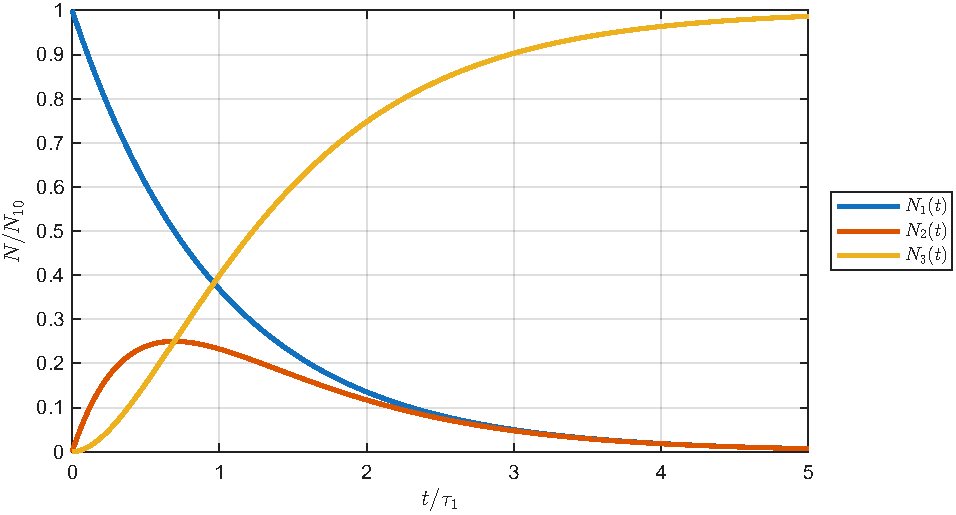
\includegraphics[width=0.8\linewidth]{figures/decay2.pdf}
		\captionof{figure}{两代连续衰变中$N_i\vs t$变化($\lambda_1/\lambda_2=1/2$)}
		\label{fig:decay2}
	\end{center}

	\tcblower

	对于$n$代连续放射性衰变过程:
	\[
		\nuc A_1\decayto{\lambda_1}\nuc A_2\decayto{\lambda_2}\cdots\decayto{\lambda_n}\nuc A_{n+1}\stable
	\]
	满足
	\begin{equation}
		\dd t
		\begin{bmatrix}
			N_1\\N_2\\\vdots\\N_n\\N_{n+1}
		\end{bmatrix}
		=
		\begin{bmatrix}
			-\lambda_1\\
			\lambda_1&-\lambda_2\\
			&\ddots&\ddots\\
			&&\lambda_{n-1}&-\lambda_n\\
			&&&\lambda_n
		\end{bmatrix}
		\begin{bmatrix}
			N_1\\N_2\\\vdots\\N_n\\N_{n+1}
		\end{bmatrix}.
	\end{equation}
	初始条件:$N_1(0)=N_{10},N_2(0)=\cdots=N_{n+1}(0)=0$,
	解得
	\begin{equation}
		N_i(t)=N_{10}\sum_{j=1}^i c_j\e{-\lambda_jt},\quad c_j=\division{\prod_{k=1}^{i-1}\lambda_k}{\prod_{k\neq j}(\lambda_k-\lambda_j)}.
	\end{equation}
	对于有分支的衰变,矩阵还需考虑分支比。
\end{example}

\paragraph{放射性平衡}

考虑两次连续衰变,经过一定时间衰变会形成平衡。根据式\eqref{eq:decay2 N2},$N_2,A_2$存在极大值:
\begin{equation}
	\dv{N_2}t=0,\implies t_\mathrm m=\frac{\ln\lambda_2-\ln\lambda_1}{\lambda_2-\lambda_1}.
\end{equation}
当$t=t_\mathrm m$时,$A_1=A_2$子母核活度相同。

\begin{definition}
	{暂时平衡}{}
	子母核的半衰期满足$T_2<T_1\lessapprox$观测时间,即母核活度在观测时间内会明显变化,如:
	\[
		\nucli{200}{Pt}\decayto[\SI{12.6}{h}]{\beta^-}\nucli{200}{Au}\decayto[\SI{48.8}{min}]{\beta^-}\nucli{200}{Hg}\stable.
	\]
	% $t>t_\mathrm m$时,$A_1<A_2$;
	经过足够长的时间($t\gg t_\mathrm m$),会形成暂时平衡\index{暂时平衡}:
	子母核数目比和活度比固定:
	\begin{equation}
		\frac{N_2}{N_1}\doteq\frac{\lambda_1}{\lambda_2-\lambda_1},\quad\frac{A_2}{A_1}\doteq\frac{\lambda_2}{\lambda_2-\lambda_1}>1.
	\end{equation}
	% 或者说子核按照母核的半衰期衰减。
\end{definition}

\begin{definition}
	{长期平衡}{}
	\index{长期平衡}
	母核半衰期$T_1\gg T_2$,虽然形式与暂时平衡相同,但平衡时子母核活度相同:
	\begin{equation}
		\frac{A_2}{A_1}\doteq\frac{\lambda_2}{\lambda_2-\lambda_1}\doteq 1.
	\end{equation}
\end{definition}

\begin{definition}
	{不成平衡}{}
	\index{不成平衡}
	母核半衰期$T_1<T_2$,经过足够长的时间之后,母核就衰变完了,只剩下子核按自己的半衰期衰变。
\end{definition}

% 以上三种平衡均存在子母核活度关系的转折点$t_\mathrm m$,且受更短半衰期的核的影响更大。

\begin{definition}
	{放射系}{}
	地球上目前存在三个天然放射系:\index{放射系}
	\begin{subequations}
		\begin{alignat}{2}
			\text{钍系}\quad&\nuclide{232}{~90}{Th}&\quad T_{1/2}&=\SI{1.4e10}{yr},\\
			\text{铀系}\quad&\nuclide{238}{~92}{U}&\quad T_{1/2}&=\SI{4.468e9}{yr},\\
			\text{锕铀系}\quad&\nuclide{235}{~92}{U}&\quad T_{1/2}&=\SI{7.038e8}{yr}.
		\end{alignat}
	\end{subequations}
	其母核的半衰期都很长,都形成了长期平衡,子核的活度与母核相同。
\end{definition}

\begin{remark}
	放射系以$_{82}$Pb为终点,导致其母核$_{84}$Po半衰期一般都很短。
\end{remark}

\section{放射规律的一些应用}

\paragraph{放射源活度修正}

$A(t)=A(0)\e{-\lambda t}=\lambda N(0)\e{-\lambda t}.$

\paragraph{确定放射源性质}

略,见讲义

\paragraph{确定放射源活度和制备时间}

人工制备放射源时,如何确定源的活度和最佳制备时间?例
\[
	\nton+\nuc A\to\nuc B+\gamma,
\]
若粒子束的强度是一定的,则放射性核素B的产生率是恒定不变的:
\begin{align}
	P=N_{\mathrm{target}}\sigma_0\Phi,
\end{align}
式中$N_{\mathrm{target}}$是靶核A的数量,$\sigma_0$表示$\nton$与A的反应截面,$\Phi$表示中子注量率($\si{1/cm^2\cdot s}$)。
故
\[
	\dv Nt=P-\lambda N(t),
\]
故源的活度应为
\begin{align}
	A(t)=P(1-\e{-\lambda t}).
\end{align}
与$N_{\mathrm{target}},\sigma_0,\Phi,\lambda,t$五个因素有关。
定义饱和因子$S:=1-\e{-\lambda t}$。\index{饱和因子}

\paragraph{放射性鉴年法}

$\nucli{14}C$具有$\beta^-$放射性,半衰期5700年。
\[
	\nucli{14}C\to\nucli{14}N+\elc^-+\bar\nu_\elc,
\]
而宇宙射线一直与大气层中的核发生反应,产生中子
\[
	\nton+\nucli{14}N\to\nucli{14}C+\pton.
\]
大气与生物体中$\nucli{12}C/\nucli{14}C$比例是一定的。生物死后体内$\nucli{14}C$不断衰变。
\paragraph{短寿命核素发生器}

核医学需要短寿命放射性核素作为标记核素,可以利用“母牛”生产这些核素并运输到医院等需要使用的地方。比如
\[
	\nucli{99}{Mo}\decayto[\SI{66}{h}]{\beta^-}\nucli{99m}{Tc}\decayto[\SI{6}{h}]{\mathrm{IT}}\nucli{99}{Tc},
\]
$t_\mathrm m=\SI{20.8}{h}$时,子核放射性活度最大,淋洗交换柱。

